% Created by tikzDevice version 0.12.6 on 2024-01-27 11:17:21
% !TEX encoding = UTF-8 Unicode
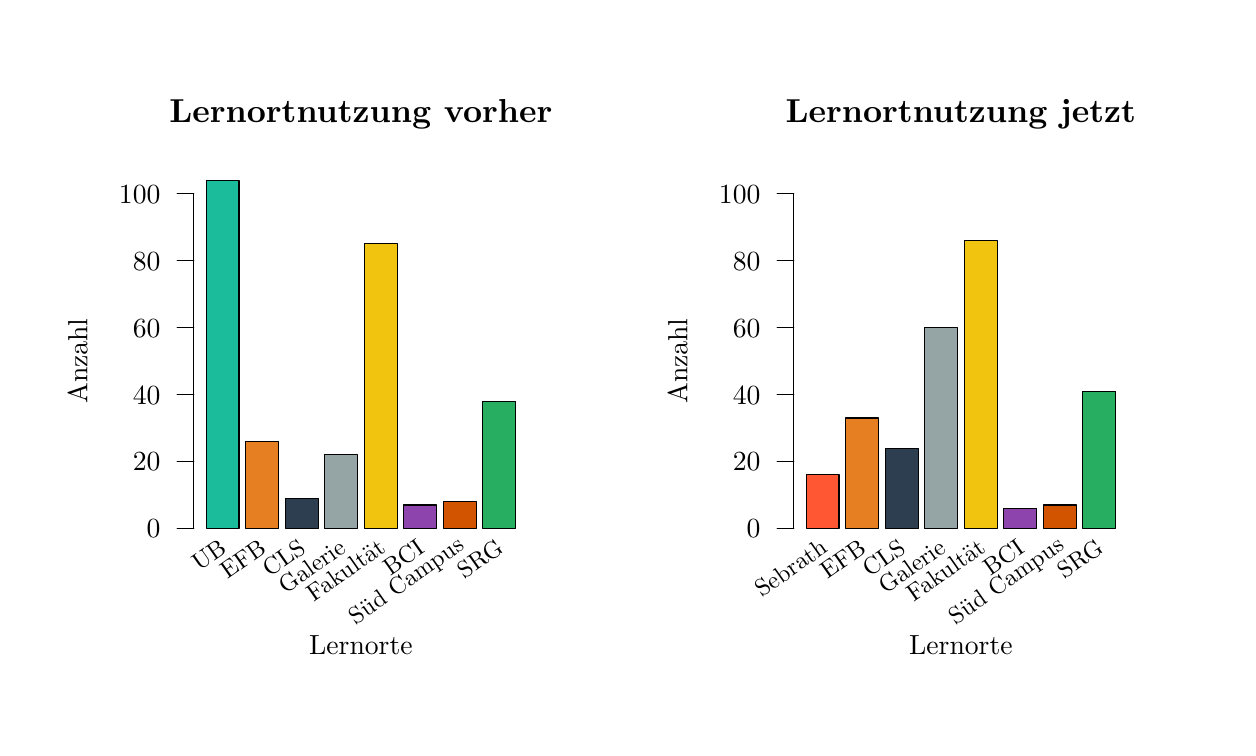
\begin{tikzpicture}[x=1pt,y=1pt]
\definecolor{fillColor}{RGB}{255,255,255}
\path[use as bounding box,fill=fillColor,fill opacity=0.00] (0,0) rectangle (433.62,252.94);
\begin{scope}
\path[clip] (  0.00,  0.00) rectangle (216.81,252.94);
\definecolor{drawColor}{RGB}{0,0,0}
\definecolor{fillColor}{RGB}{26,188,156}

\path[draw=drawColor,line width= 0.4pt,line join=round,line cap=round,fill=fillColor] ( 64.47, 72.00) rectangle ( 76.37,197.78);
\definecolor{fillColor}{RGB}{230,126,34}

\path[draw=drawColor,line width= 0.4pt,line join=round,line cap=round,fill=fillColor] ( 78.75, 72.00) rectangle ( 90.65,103.45);
\definecolor{fillColor}{RGB}{44,62,80}

\path[draw=drawColor,line width= 0.4pt,line join=round,line cap=round,fill=fillColor] ( 93.03, 72.00) rectangle (104.93, 82.89);
\definecolor{fillColor}{RGB}{149,165,166}

\path[draw=drawColor,line width= 0.4pt,line join=round,line cap=round,fill=fillColor] (107.31, 72.00) rectangle (119.21, 98.61);
\definecolor{fillColor}{RGB}{241,196,15}

\path[draw=drawColor,line width= 0.4pt,line join=round,line cap=round,fill=fillColor] (121.60, 72.00) rectangle (133.50,174.80);
\definecolor{fillColor}{RGB}{142,68,173}

\path[draw=drawColor,line width= 0.4pt,line join=round,line cap=round,fill=fillColor] (135.88, 72.00) rectangle (147.78, 80.47);
\definecolor{fillColor}{RGB}{211,84,0}

\path[draw=drawColor,line width= 0.4pt,line join=round,line cap=round,fill=fillColor] (150.16, 72.00) rectangle (162.06, 81.68);
\definecolor{fillColor}{RGB}{39,174,96}

\path[draw=drawColor,line width= 0.4pt,line join=round,line cap=round,fill=fillColor] (164.44, 72.00) rectangle (176.34,117.96);

\node[text=drawColor,anchor=base,inner sep=0pt, outer sep=0pt, scale=  1.20] at (120.40,218.80) {\bfseries Lernortnutzung vorher};

\node[text=drawColor,anchor=base,inner sep=0pt, outer sep=0pt, scale=  1.00] at (120.40, 26.40) {Lernorte};

\node[text=drawColor,rotate= 90.00,anchor=base,inner sep=0pt, outer sep=0pt, scale=  1.00] at ( 21.60,132.47) {Anzahl};
\end{scope}
\begin{scope}
\path[clip] (  0.00,  0.00) rectangle (433.62,252.94);
\definecolor{drawColor}{RGB}{0,0,0}

\path[draw=drawColor,line width= 0.4pt,line join=round,line cap=round] ( 60.00, 72.00) -- ( 60.00,192.94);

\path[draw=drawColor,line width= 0.4pt,line join=round,line cap=round] ( 60.00, 72.00) -- ( 54.00, 72.00);

\path[draw=drawColor,line width= 0.4pt,line join=round,line cap=round] ( 60.00, 96.19) -- ( 54.00, 96.19);

\path[draw=drawColor,line width= 0.4pt,line join=round,line cap=round] ( 60.00,120.38) -- ( 54.00,120.38);

\path[draw=drawColor,line width= 0.4pt,line join=round,line cap=round] ( 60.00,144.57) -- ( 54.00,144.57);

\path[draw=drawColor,line width= 0.4pt,line join=round,line cap=round] ( 60.00,168.76) -- ( 54.00,168.76);

\path[draw=drawColor,line width= 0.4pt,line join=round,line cap=round] ( 60.00,192.94) -- ( 54.00,192.94);

\node[text=drawColor,anchor=base east,inner sep=0pt, outer sep=0pt, scale=  1.00] at ( 48.00, 68.56) {0};

\node[text=drawColor,anchor=base east,inner sep=0pt, outer sep=0pt, scale=  1.00] at ( 48.00, 92.75) {20};

\node[text=drawColor,anchor=base east,inner sep=0pt, outer sep=0pt, scale=  1.00] at ( 48.00,116.93) {40};

\node[text=drawColor,anchor=base east,inner sep=0pt, outer sep=0pt, scale=  1.00] at ( 48.00,141.12) {60};

\node[text=drawColor,anchor=base east,inner sep=0pt, outer sep=0pt, scale=  1.00] at ( 48.00,165.31) {80};

\node[text=drawColor,anchor=base east,inner sep=0pt, outer sep=0pt, scale=  1.00] at ( 48.00,189.50) {100};

\node[text=drawColor,rotate= 35.00,anchor=base east,inner sep=0pt, outer sep=0pt, scale=  0.87] at ( 72.35, 63.64) {UB};

\node[text=drawColor,rotate= 35.00,anchor=base east,inner sep=0pt, outer sep=0pt, scale=  0.87] at ( 86.71, 63.70) {EFB};

\node[text=drawColor,rotate= 35.00,anchor=base east,inner sep=0pt, outer sep=0pt, scale=  0.87] at (100.97, 63.69) {CLS};

\node[text=drawColor,rotate= 35.00,anchor=base east,inner sep=0pt, outer sep=0pt, scale=  0.87] at (115.43, 63.81) {Galerie};

\node[text=drawColor,rotate= 35.00,anchor=base east,inner sep=0pt, outer sep=0pt, scale=  0.87] at (129.79, 63.87) {Fakultät};

\node[text=drawColor,rotate= 35.00,anchor=base east,inner sep=0pt, outer sep=0pt, scale=  0.87] at (143.80, 63.68) {BCI};

\node[text=drawColor,rotate= 35.00,anchor=base east,inner sep=0pt, outer sep=0pt, scale=  0.87] at (158.13, 64.75) {Süd Campus};

\node[text=drawColor,rotate= 35.00,anchor=base east,inner sep=0pt, outer sep=0pt, scale=  0.87] at (172.40, 63.70) {SRG};
\end{scope}
\begin{scope}
\path[clip] (216.81,  0.00) rectangle (433.62,252.94);
\definecolor{drawColor}{RGB}{0,0,0}
\definecolor{fillColor}{RGB}{255,87,51}

\path[draw=drawColor,line width= 0.4pt,line join=round,line cap=round,fill=fillColor] (281.28, 72.00) rectangle (293.18, 91.35);
\definecolor{fillColor}{RGB}{230,126,34}

\path[draw=drawColor,line width= 0.4pt,line join=round,line cap=round,fill=fillColor] (295.56, 72.00) rectangle (307.46,111.91);
\definecolor{fillColor}{RGB}{44,62,80}

\path[draw=drawColor,line width= 0.4pt,line join=round,line cap=round,fill=fillColor] (309.84, 72.00) rectangle (321.74,101.03);
\definecolor{fillColor}{RGB}{149,165,166}

\path[draw=drawColor,line width= 0.4pt,line join=round,line cap=round,fill=fillColor] (324.12, 72.00) rectangle (336.02,144.57);
\definecolor{fillColor}{RGB}{241,196,15}

\path[draw=drawColor,line width= 0.4pt,line join=round,line cap=round,fill=fillColor] (338.41, 72.00) rectangle (350.31,176.01);
\definecolor{fillColor}{RGB}{142,68,173}

\path[draw=drawColor,line width= 0.4pt,line join=round,line cap=round,fill=fillColor] (352.69, 72.00) rectangle (364.59, 79.26);
\definecolor{fillColor}{RGB}{211,84,0}

\path[draw=drawColor,line width= 0.4pt,line join=round,line cap=round,fill=fillColor] (366.97, 72.00) rectangle (378.87, 80.47);
\definecolor{fillColor}{RGB}{39,174,96}

\path[draw=drawColor,line width= 0.4pt,line join=round,line cap=round,fill=fillColor] (381.25, 72.00) rectangle (393.15,121.59);

\node[text=drawColor,anchor=base,inner sep=0pt, outer sep=0pt, scale=  1.20] at (337.21,218.80) {\bfseries Lernortnutzung jetzt};

\node[text=drawColor,anchor=base,inner sep=0pt, outer sep=0pt, scale=  1.00] at (337.21, 26.40) {Lernorte};

\node[text=drawColor,rotate= 90.00,anchor=base,inner sep=0pt, outer sep=0pt, scale=  1.00] at (238.41,132.47) {Anzahl};
\end{scope}
\begin{scope}
\path[clip] (  0.00,  0.00) rectangle (433.62,252.94);
\definecolor{drawColor}{RGB}{0,0,0}

\path[draw=drawColor,line width= 0.4pt,line join=round,line cap=round] (276.81, 72.00) -- (276.81,192.94);

\path[draw=drawColor,line width= 0.4pt,line join=round,line cap=round] (276.81, 72.00) -- (270.81, 72.00);

\path[draw=drawColor,line width= 0.4pt,line join=round,line cap=round] (276.81, 96.19) -- (270.81, 96.19);

\path[draw=drawColor,line width= 0.4pt,line join=round,line cap=round] (276.81,120.38) -- (270.81,120.38);

\path[draw=drawColor,line width= 0.4pt,line join=round,line cap=round] (276.81,144.57) -- (270.81,144.57);

\path[draw=drawColor,line width= 0.4pt,line join=round,line cap=round] (276.81,168.76) -- (270.81,168.76);

\path[draw=drawColor,line width= 0.4pt,line join=round,line cap=round] (276.81,192.94) -- (270.81,192.94);

\node[text=drawColor,anchor=base east,inner sep=0pt, outer sep=0pt, scale=  1.00] at (264.81, 68.56) {0};

\node[text=drawColor,anchor=base east,inner sep=0pt, outer sep=0pt, scale=  1.00] at (264.81, 92.75) {20};

\node[text=drawColor,anchor=base east,inner sep=0pt, outer sep=0pt, scale=  1.00] at (264.81,116.93) {40};

\node[text=drawColor,anchor=base east,inner sep=0pt, outer sep=0pt, scale=  1.00] at (264.81,141.12) {60};

\node[text=drawColor,anchor=base east,inner sep=0pt, outer sep=0pt, scale=  1.00] at (264.81,165.31) {80};

\node[text=drawColor,anchor=base east,inner sep=0pt, outer sep=0pt, scale=  1.00] at (264.81,189.50) {100};

\node[text=drawColor,rotate= 35.00,anchor=base east,inner sep=0pt, outer sep=0pt, scale=  0.87] at (289.44, 63.84) {Sebrath};

\node[text=drawColor,rotate= 35.00,anchor=base east,inner sep=0pt, outer sep=0pt, scale=  0.87] at (303.52, 63.70) {EFB};

\node[text=drawColor,rotate= 35.00,anchor=base east,inner sep=0pt, outer sep=0pt, scale=  0.87] at (317.78, 63.69) {CLS};

\node[text=drawColor,rotate= 35.00,anchor=base east,inner sep=0pt, outer sep=0pt, scale=  0.87] at (332.24, 63.81) {Galerie};

\node[text=drawColor,rotate= 35.00,anchor=base east,inner sep=0pt, outer sep=0pt, scale=  0.87] at (346.60, 63.87) {Fakultät};

\node[text=drawColor,rotate= 35.00,anchor=base east,inner sep=0pt, outer sep=0pt, scale=  0.87] at (360.61, 63.68) {BCI};

\node[text=drawColor,rotate= 35.00,anchor=base east,inner sep=0pt, outer sep=0pt, scale=  0.87] at (374.94, 64.75) {Süd Campus};

\node[text=drawColor,rotate= 35.00,anchor=base east,inner sep=0pt, outer sep=0pt, scale=  0.87] at (389.21, 63.70) {SRG};
\end{scope}
\end{tikzpicture}
